\hyperref[sec:sec34]{\section{為什麼立法會議員只懂批評不會建設?}}
\label{sec:sec21}

因為香港的政治制度要求立法會議員多批評,不要求也不鼓勵他們懂建設。上文提到行政長官施政舉步維艱的其中一個原因,是難以在立法會中得到支持。不過,這並不等於立法會在香港政制中的權力就十分巨大。相反,香港的政制在設計上阻礙行政長官的同時,也使得立法會未能發揮一個立法機關應有的角色。相對於責怪行政和立法互拉後腿,制度上其實本來就不容許兩者有效運作。

前文提到由於制度上的缺陷,行政長官的民意支持度總體來說只會跌、不會升。然而在行政長官支持度和認授低落的同時,作為監督者的立法會卻沒有因而受惠,支持度和認授同樣低落,兩者彷如競逐民意下限。當中的原因,在於立法會在設計上的功能就被嚴重限制,而過上限制使得其工作不被重視,立法會漸漸變成政治表演的場所,而這個趨向又反過來拖累政府的正常運作。

香港立法會和世界各地的議會一樣,首要功能固然是要代表民意。不過香港立法會無論是選舉方式和議事制度,都使它無法好好發揮民意代表的功能。現時香港立法會有七十個議席,當中一半由地區直選產生,另一半由功能界別產生。所謂功能界別,很大程度上和行政長官選舉中的選舉委員會相重疊。選舉委員會中有漁農界、保險界和法律界,立法會功能界別當中一樣有漁農界、保險界和法律界。不同的地方,在於每個界別選舉委員會中所佔的席數不一,但在立法會當中則一般只有一席。

功能界別的出現正正是立法會不能「好好議事」的一個重要原因,因為它大幅扭曲了立法會的代表性。前文談及所有選舉委員會的制度問題,在立法會功能界別當中同樣適用:一)界別的成立沒有客觀標準;二)界別選民地位的定義沒有客觀標準;三)每個界別的代表人數差距極大;和四)大多數市民無權參與。舉個例,商界(第一)的選民只限香港總商會會員,商界(第二)的選民則只限香港中華總商會會員,其他的商人和組織都不被排除在外。因為這些限制,在二零一六年的立法會選舉中,就有十二名候選人循功能界別自動當選。回顧自特區成立以來的五屆立法會選舉,有三個界別(鄉議局、進出口界及商界(二))從來都是自動當選,一次正式競爭都沒有。自動當選的出現,代表他們的界別在選舉前已各自被不同的政治力量所壟斷,其他勢力明白就算參選也枉廢心思。換言之,功能界別的設立可確保個別政治勢能在立法會當中穩奪席位,違反民主原則。

\begin{figure}[htbp]
    \centering
    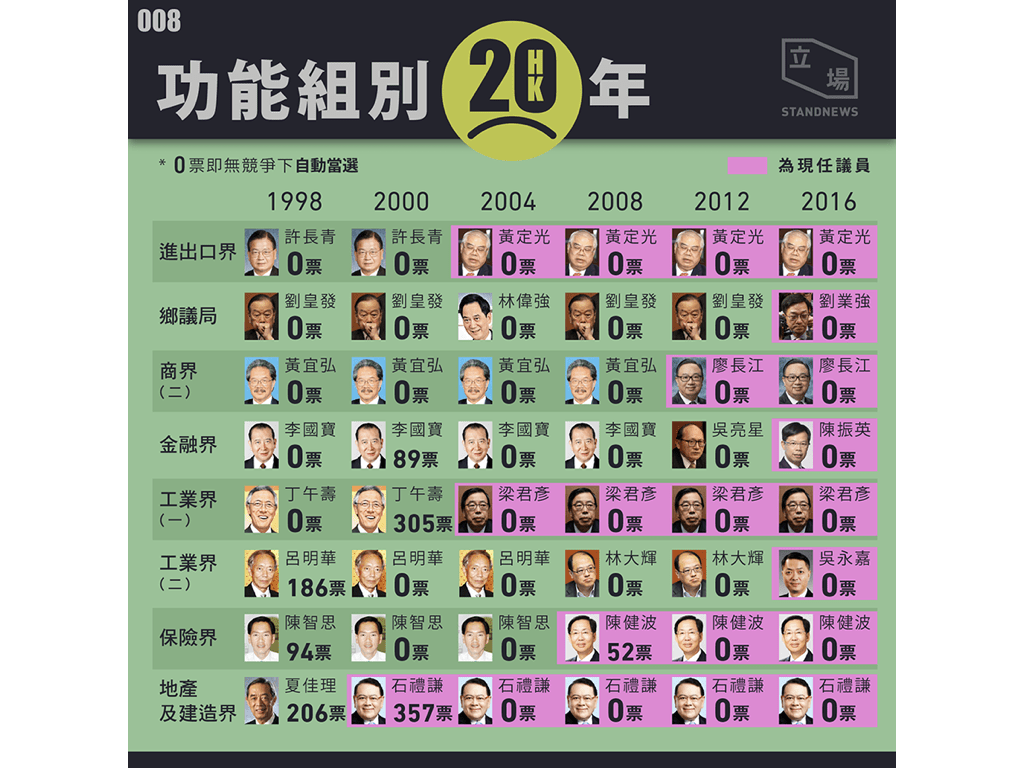
\includegraphics[width=0.7\textwidth]{c21/h-klesson1-033.png}
    \caption{不少功能組別議席均為「零票當選」,表示這些議席正正是為了保障個別政治勢力而設。} 
\end{figure}

非建制陣營在功能界別當中一般只有法律、教育、社會福利,和衛生服務界有穩定的支持,以及在少數界別有能力競爭,其餘多數界別都是建制陣營的囊中物。透過界別劃分和選民界定,功能界別成為了親政府的建制派議員在立法會保持過半數的關鍵。以二零一六年的立法會選舉為例,建制陣營在地區直選的得票為八十七萬票,佔百分之四十;非建制陣營得票為一百一十九萬票,佔百分之五十五。只看地區直選的話,建制陣營佔十六席,非建制陣營佔十九席,比例尚算合理。但再加上功能界別的議席後,則變成建制陣營佔四十席,非建制陣營佔二十九席,中間派佔一席。換言之,透過功能界別的加持,明明是非建制陣營的得票較多,大多數的議席卻會落在建制陣營之中。

這是制度設計的一部分。在訂立《基本法》的時候,中央政府很明白如果立法會全部議席由一人一票產生,他們便不能控制誰是立法會的多數派。然而透過保留功能界別以及背後的利益交易,中央政府就可以很大程度上左右立法會的派別構成。自特區成立以來,主流民意一直要求取消功能界別制度,唯自二零零四年起地區直選和功能界別的議席比例就一直都沒有改變過,維持各佔一半,政府也未能承諾最終取消功能界別。

功能界別的存在保持了建制陣營在議會的主導權,卻同時帶來一個很壞的後果:市民對立法會的期望改變。在一個正常的議會當中,選民投票選出議員時的其中一個考量,是議會的構成會如何影響議案的處理。在理性選擇的框架下,支持某項政策的選民理應投最有能力落實此政策的候選人一票,好讓他們在議會中佔多數,然後通過相關的法案。實際上的選民的考量當然會複雜很多,例如有些選民會接受他們的代表在必要時妥協,另一些的選民卻會希望他們的代表立場堅定,甚至「有破壞沒建設」,但求阻礙他們眼中的惡法通過。問題的重點,在於當選民認為他們支持的政黨或派別永遠無法成為多數的時候,選民的思考便會傾向後者多一點,對候選人能力的評估也從重視審議的能力變成破壞的能力。

香港立法會的情況正正就是這樣。因為無論一項議案在市民心目中如何的不受歡迎,建制陣營也會有足夠的票數強行通過,於是選民逐漸發現立法會不能真正議政。礙於選舉制度的不公平,即使非建制陣營在選票數目上贏得多數,也不能轉換成議席上的多數。政府也發現他們不用真的和所有的議員建立良性互動,只要通過前文論及的利益交易穩住建制陣營即可。如是者,立法會失去審議功能,選民對議員的要求也慢慢從慎思變為敢言。既然非建制陣營的議員無論提出什麼議案也不會夠票通過,對選民來說與其找一個有審議能力的人來當議員,倒不如找一個罵政府罵得精彩的人來當。反正最後任何議案的投票結果都會一樣,但有議員代表自己直接在議事堂內罵官員,而這些官員在制度上又要被迫接受這些質詢,也算是幫大家出一口氣。議員當然也很明白這個趨勢,眼見政府可以主導立法會的工作,議員剩下來的功能就只有提出反對;當一個表演精彩的反對派來吸引選民注意,就成為連任的本錢。在這畸形的選舉制度下,立法會便變成一個政治表演的地方。

選舉制度外,立法會的議事制度也不容許有建設性意見的人帶來政策創新。《基本法》第七十四條這樣規定:

\begin{displayquote}
    香港特別行政區立法會議員根據本法規定並依照法定程序提出法律草案,凡不涉及公共開支或政治體制或政府運作者,可由立法會議員個別或聯名提出。凡涉及政府政策者,在提出前必須得到行政長官的書面同意。
\end{displayquote}

這條條文等如完全廢除了立法會的提案權。畢竟如果政府本身想做,政府自己會在立法會提出,不會給議員有機會領功。當一件事情政府本身不想做,議員將不能通過立法會的議決強迫政府去做的,因為他們連提案的機會也沒有。因此,坊間有時會批評議員們「有破壞沒建設」,事實上是立法會的制度不容許也不鼓勵他們有任何建設。而由於選舉制度讓建制陣營容易控制立法會的主導權,所以即使有議員不滿政府的提案,也不能通過拉攏其他議員來合力否決,而只能在電視直播辯論的時候表達完不滿,然後便沒有然後了。

雖然如此,仍有議員會嘗試提出「私人條例草案」,一方面促使政府正視議題,同時也向選民顯示他們對議題的理解。近年的例子,就有《災難狀態條例草案》和《罕見疾病防治、藥物及支援條例》等。

此外,政府還有各種方法繞過立法會的監督權。政府的開支須獲立法會財務委員會審批,而由於建制陣營的議員佔多數,政府的撥款申請幾乎都會獲得通過。不過,非建制陣營最起碼能在辯論的過程提出質疑,引起公眾關注。然而近年來,政府發現既然每一次提出撥款申請,就要面對一次質疑,無論是要一億、十億還是一百億也一樣,倒不如把各項開支都放在同一個撥款中一併申請,減少了立法會可逐項討論這些開支的機會。以關愛基金為例,政府先後向立法會申請注資二百億元,而基金的日常運作則由督導委員會負責,立法會便先去了直接監督的能力。另一種做法,則是通過不直接動用庫房的手段融資。以機場三跑系統為例,儘管估算造價超過一千四百億元,卻無須立法會審議通過。機場管理局通過向銀行借貸發債、未來十年暫停向政府發放股息,以及向旅客及航空公司徵費的手段籌措資金。雖然這些做法實際上會減少政府的財政收入,卻因沒有直接動用庫房而繞過了立法會的監督。

議員要突破這些限制的空間十分有限,而且往往要採用迂回的手法來提出質疑。例如議員雖然不能要求增加開支,卻可以要求減少開支,於是乎每一次的財政預算案辯論都會有一系列要求削減撥款的修正案。這些修正案一般都無望通過,議員提出的目的是要把他們關心的問題帶上議程,強迫政府回應。例如有議員反對漁護署處理流浪動物的做法,便提出削減漁護署的相關開支;有議員不滿個別問責官員的表現,便要求削減他們來年的人工。不過這樣做也有一定風險,例如有議員曾經要求削減消防署開支,原因並不是他們真的反對這些開支,而是認為撥款的程序有問題。但當發生重大火災之後,某些刻意誤導的輿論一樣會翻他們的舊帳,批評他們不支持消防署的工作。

另一個議員發聲的方法,是提出沒有約束力的議案,來繞過《基本法》第七十四條的限制。但這個方法的實際功能也很有限。首先,這些議案由於沒有約束力,就算通過了政府也可以不理。再者,這條進路還要面對《基本法》附件二的另一頂要求:

\begin{displayquote}
    政府提出的法案,如獲得出席會議的全體議員的過半數票,即為通過。
    
    立法會議員個人提出的議案、法案和對政府法案的修正案均須分別經功能團體選舉產生的議員和分區直接選舉、選舉委員會選舉產生的議員兩部分出席會議議員各過半數通過。
\end{displayquote}

這項條文一般稱之為「分組點票」,即議員自己提出的議案不單要得到立法會的過半數通過,還要分別獲過半地區直選選出的議員和過半功能界別選出的議員通過,才算是通過。由於地區直選選出的議員通常傾向非建制陣營,而功能界別選出的議員通常傾向建制陣營,兩者目標一致的情況並不常見,所以這些議案往往很難獲得通過。

自特區成立以來,就有很多議案雖然獲得過半數議員支持,卻在「分組點票」之下被否決。特別是以保護勞工和低下階層為目標的議案,既得利益就往往可以利用工商界在功能界別的優勢,把「分組點票」變成他們的專屬否決權。就算所有議員都出席會議,只要四分之一的議員便足以否決四分之三多數議員的意願;最極端的情況下,甚至可以只有一名議員反對便能否決議案。在這樣的安排下,立法會否決議案的機會就變得高於通過議案,同樣成為立法會「有破壞沒建設」的制度原由。以二零零五年的「最低工資、標準工時」議案為例,雖然總票數為三十六票贊成,十七票否決,但是議案在「分組點票」下仍被否決。出現此結果,是因為議案於地區直選議席的表決結果是二十五比二,但於功能界別議席則是十一比十五,由於未能獲功能界別議席通過而被否決。

\begin{figure}[htbp]
    \centering
    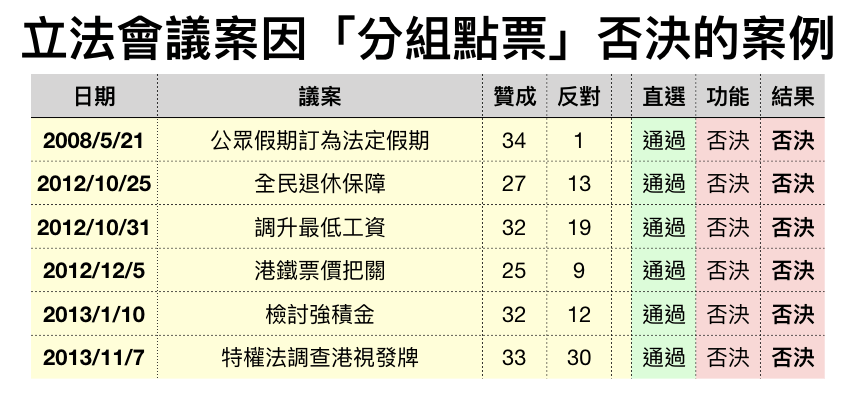
\includegraphics[width=0.7\textwidth]{c21/h-klesson1-034.png}
    \caption{「分組點票」導致多數議員贊成的議案無法通過} 
\end{figure}

值得注意的,是「分組點票」是只限於議員提出的議案,由政府提出的則沒此限制。所以,正常來說非建制陣營會較受影響,因為建制陣營本來就是政府「執政聯盟」的一部分,議案可直接由政府提出,不受非建制陣營在地區直選的優勢影響。按香港大學於二零一三年的民意調查所得,有四成六的受訪者贊成取消「分組點票」,反對者只有一成半,民意明顯不認同「分組點票」的安排。

「分組點票」帶來的另一個問題,是立法會無法有效利用《立法會(權力及特權)條例》(又稱《特權法》)提供的調查權。《特權法》的設立是要保障立法會議員的權力,例如出席會議時可免受刑事逮捕,不會因議會發言內容被提出訴訟等。《特權法》其中一個稱為「尚方寶劍」的權力,是可以傳召任何人作證或出示其所管有或控制的任何文件,甚至要求警察拘捕證人強迫列席作證,可以說是議會監督政府的最後防線。不過,此項權力在特區成立以來只被引用過六次。由於《特權法》調查要「分組點票」組過,不少評論質疑只要少數議員為了保護其政治利益而反對,調查就無法立項。

說到這兒,得同時指出建制陣營把持立法會帶來的另一個效果:為免政府尷尬,有時立法會連提意見的機會也沒有。如要在立法會的日常議程外加入討論社會中的突發狀況,要先得到主席批准,而在現有的立法會構成下無論是大會或各委員會的主席都是由建制陣營的議員出任。主席的各種裁決能力可使得立法會本來可用作監督政府的權力無從發揮。如果說現在的立法會沒有好好議事,則得先明白立法會的議事權本身已被自我閹割。

話雖如此,即使在這麼有限的空間之下,立法會議員也不是完全無事可做。舉個例,議員仍可通過質詢要求政府回答問題,公開重要的公共信息。這些工作雖然未能直接解決問題,但借立法會這個平台來揭發問題和引發公眾關注,本身已經十分重要。而在電視直播的質詢過程中令政府官員尷尬,也可迫使政府作出一定程度的檢討和改善。今天的香港立法會雖然距離一個真正的民主議會甚遠,但也未至於完全無能。

儘管《基本法》沒有直接用上「三權分立」這四個字,但從條文上可以清楚看到政府的職能被放在不同的機構當中,以發揮互相監督和平衡的角色:行政機關執行決策,立法機關監督決策執行,而司法機關又可以監督行政機關和立法機關。三者之間的互動如能有效實行的話,可避免政府變成一言堂,不得民心的做法有機會被修正。所以,立法會議員質詢政府官員,只不過是在履行其職責所在。事實上,現在立法會議員要有效地質詢政府官員已經十分困難。

總的來說,「立法會議員只懂批評不會建設」的說法其實是一種錯覺。事實上,考慮到香港立法會在制度上的種種限制,議員們有時看似激烈的抗爭手法其實有十分理性的制度原由。如果說立法會議員的議政質素未如理想,則得明白在香港的畸型政治制度下,在朝的永遠在朝,在野的永遠在野。所以,在朝者其實沒有誘因提高其議政能力,只用做橡皮圖章就行;在野的也難以尋找人才放棄他們原來的生活,投身於勞而不獲的抗爭。反過來說,如果希望議會政治變得更專業,不能只責怪個別議員甚至政黨的表現,而要改變整個議會制度,包括選舉和議事制度,理順議會的權責,才能為改變議會文化提供基礎。

立法會整天吵吵鬧鬧只是病徵,意圖通過修改會議規則或驅逐議員來解決只是針對病徵而非病因。畢竟,病徵去除不等於問題消失,也可能是因為病人死亡。正確的回應應該是對症下藥,從制度病因著手。

\rule[-10pt]{15cm}{0.05em}

伸延閱讀:

馬嶽(2013):《港式法團主義:功能界別25年》,香港:香港城市大學出版社。

許寶強(2010):〈議會難言「理性」 「激進」原是認真〉,《明報》2010年1月24日。

Lui PLT (2012) The Legislature, Contemporary Hong Kong Government and Politics (Expanded Edition). Hong Kong University Press.

網上資源:

\href{https://thestandnews.com/politics/圖析香港主權移交20年/}{圖析新聞(2017):〈圖析香港主權移交20年〉:立場新聞,2017年6月30日}
